\documentclass{beamer}
\usepackage{amsmath}
\usepackage{textcomp}
\usepackage{lmodern}
\usepackage[T1]{fontenc}
\usepackage{quiver}
\usepackage{biblatex}

\addbibresource{biblio.bib}

\usetheme{Berlin}

\newtheorem{proposition}{Proposition}

\DeclareMathOperator{\im}{im}
\DeclareMathOperator{\id}{id}

\newcommand{\NN}{\mathbb{N}}
\newcommand{\ZZ}{\mathbb{Z}}
\newcommand{\cat}[1]{\mathsf{#1}}

\title{An Introduction to Abelian Categories}

% Reduce vertical space between author and date
\author{Gabriel Antonio Videtta\texorpdfstring{\vspace*{-13pt}}{}}

\date{May 2025}
\logo{
\includegraphics[width=0.7cm]{unipi_logo.png}}

\titlegraphic{
    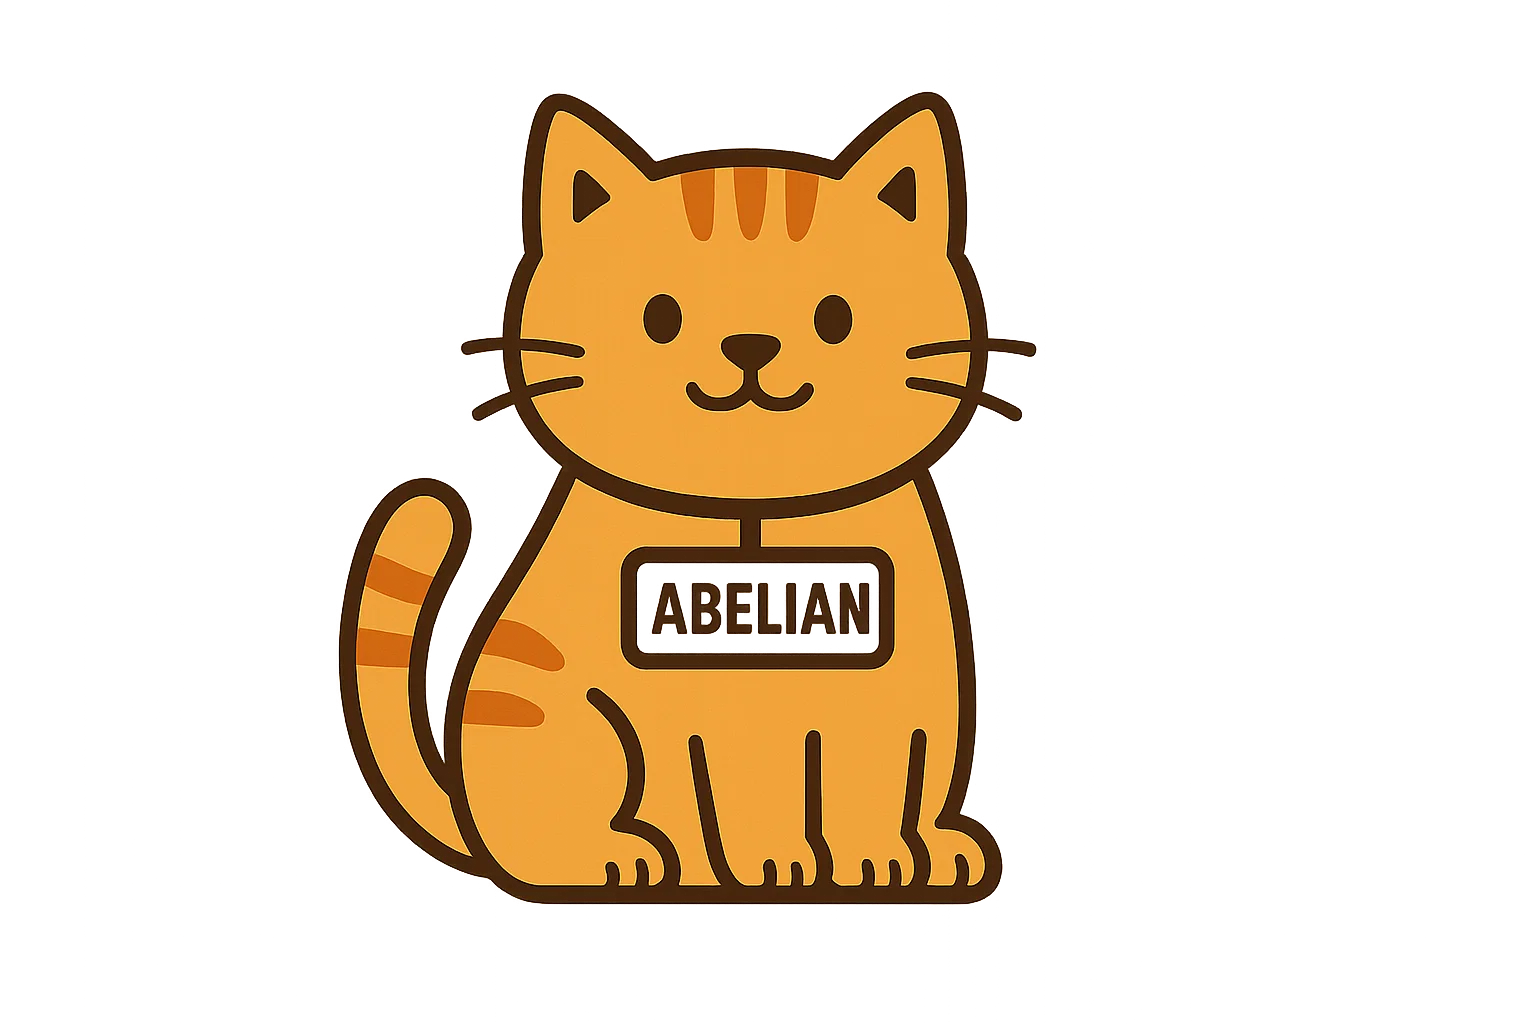
\includegraphics[width=4cm]{abelian_cat.jpg}
}

% Hack from https://latex.org/forum/viewtopic.php?t=2387
% Allows to show only the current section in the Berlin theme
\makeatletter
\renewcommand*\insertnavigation[1]{%
  \vbox{{%
    \usebeamerfont{section in head/foot}\usebeamercolor[fg]{section in head/foot}%
    \beamer@xpos=0\relax%
    \beamer@ypos=1\relax%
    \hskip.3cm\setbox\beamer@sectionbox=\hbox{\kern1sp}%
      \ht\beamer@sectionbox=1.875ex%
      \dp\beamer@sectionbox=0.75ex%
        \insertsectionhead%
      \box\beamer@sectionbox\hfil\hskip.3cm%
  }}}
\makeatother

\begin{document}

\begin{frame}
    \titlepage
\end{frame}


\begin{frame}{Outline}
    \tableofcontents
\end{frame}

\AtBeginSection[ ]
{
\begin{frame}{Outline}
    \tableofcontents[currentsection]
\end{frame}
}

%%%
% Background: Abelian Groups, K-Vector Spaces and R-Modules
%%%

\section{Background: Abelian Groups, \texorpdfstring{$K$}{K}-Vector Spaces, and \texorpdfstring{$R$}{R}-Modules}

\begin{frame}
    Before we take a look at abelian categories, we
    need to introduce the algebraic structure they
    all rely on: \textbf{abelian groups}. \medskip

    \begin{definition}[Abelian group]
        An abelian group $(G, +)$ is a commutative monoid
        which allows inverses.
    \end{definition}

    Abelian groups are fairly simple objects with respect to what
    a general non-commutative group might be. Nonetheless, they
    appear everywhere: $\ZZ$ and the integers modulo $n$ form
    an abelian group with addition, and all vector spaces rely on
    abelian groups for their additive structure.
\end{frame}

\begin{frame}
    In fact, the connection between vector spaces and abelian groups is
    deeper than what it initially appears to be. In order to show this,
    let us recall the definition of a \textbf{ring} and of a \textbf{module}.

    \begin{definition}[Ring]
        A ring is a set $R$ equipped with two binary operations $+$ and $\cdot$
        such that $(R, +)$ is an abelian
        group, $(R, \cdot)$ is a monoid and law of distributivity applies, i.e.
        for any choice of $a$, $b$, $c \in R$
        \[
            a \cdot (b + c) = a \cdot b + a \cdot c,
        \]
        \[
            (a + b) \cdot c = a \cdot c + b \cdot c.
        \]
    \end{definition}
\end{frame}

\begin{frame}
    \begin{definition}[$R$-module]
        Given a ring $R$, we say that a set $A$ equipped with a binary operation $+$ is an $R$-module with
        scalar multiplication $\cdot$ if:
        \begin{enumerate}
            \item $(A, +)$ is an abelian group,
            \item $1 \cdot a = a$, where $1$ is the unity of the ring $R$ and $a \in A$,
            \item $\lambda \cdot (\mu \cdot a) = (\lambda \cdot \mu) \cdot a$, for each $\lambda$, $\mu \in R$, and $a \in A$, 
            \item $(\lambda + \mu) \cdot a = \lambda \cdot a + \mu \cdot a$ for each $\lambda$, $\mu \in R$, and $a \in A$,
            \item $\lambda \cdot (a + b) = \lambda \cdot a + \lambda \cdot b$ for each $\lambda \in R$, and $a$, $b \in A$.
        \end{enumerate}
    \end{definition}
\end{frame}

\begin{frame}
    In this setting, $K$-vector spaces are simply $K$-modules and abelian groups
    are simply $\ZZ$-modules with the following scalar multiplication:
    \[
        k \cdot g \triangleq \begin{cases}
            \underbrace{g + \ldots + g}_{k \text{ times}} & k \geq 0 \\
            -(-k) \cdot g & k < 0.
        \end{cases}
    \] \smallskip

    Modules are indeed a great unifying concept for these two algebraic structure, and we'll see
    at the end of the presentation that the Freyd-Mitchell's embedding theorem will
    give us more reasons to believe so.
\end{frame}

%%%
% Origins and Motivation of Abelian Categories
%%%

\section{Origins and Motivation of Abelian Categories}

\begin{frame}
    In 1945 two mathematicians, Eilenberg and Mac Lane, wrote for the
    first time about categories in the way we look at them now. \medskip
    
    They were looking to
    deeply understand \textit{natural transformations}, hence they had
    to deal with functors and categories first. Their goal was to
    apply such abstractness to homological algebra, which revolves
    around \textbf{chain complexes}. \medskip

    Understanding chain complexes allow mathematicians to retrieve
    topological invariants from geometrical structures in a pure
    algebraic setting.
\end{frame}

\begin{frame}
    Chain complexes are particular concatenations of morphisms in $\cat{Ab}$, the
    category of abelian groups, written as seen below
    \[\begin{tikzcd}[sep=large, ampersand replacement=\&]
        {C_1} \& {C_2} \& \ldots \& {C_n}
        \arrow["{d_1}", from=1-1, to=1-2]
        \arrow["{d_2}", from=1-2, to=1-3]
        \arrow["{d_{n-1}}", from=1-3, to=1-4]
    \end{tikzcd}\]
    where $d_{i+1} \circ d_i = 0$ for each $i$ (i.e., $\im d_i \subseteq \ker d_{i+1}$). \smallskip

    We say that such a chain complex is \textbf{exact} whenever $\im d_i$ is exactly
    $\ker d_{i+1}$ for each $i$.
\end{frame}

\begin{frame}
    The goal of abelian categories is to provide the most general setting to
    generalise and make use of chain complexes. \medskip
    
    Instances of the definition of abelian
    categories are first found in a paper from 1955 by Buchsbaum, whereas further
    foundations of the theory were laid in a famous paper from
    Grothendieck later in 1957. \medskip

    The goal of this presentation is to derive the modern setting of
    abelian categories from scratch.
\end{frame}

%%%
% Derivation of Abelian Categories
%%%

\section{Derivation of Abelian Categories}

\begin{frame}
    In order to derive a correct definition for
    abelian categories, we need to address the following issues:
    \begin{enumerate}
        \item We must allow for the existance of ``zero morphisms'',
            since we want $d_{i+1} \circ d_i = 0$.
        \item We must allow some structure for the hom-sets, as
            group homomorphisms between two abelian groups $A$ and
            $B$ form an abelian group as well.
        \item We need to define kernels in a pure categorical sense,
            since $\ker f$ is defined in a set-theoretic manner. 
    \end{enumerate}
\end{frame}

\begin{frame}{Zero objects I}
    Abelian groups, vector spaces, and modules in general have a peculiar property: \textit{initial objects and
    final objects are the same!} \medskip
    
    In both cases, such initial object is always
    denoted as the ``trivial'' or ``zero'' object, since it always induces a
    ``trivial'' morphism with respect to another module.
\end{frame}

\begin{frame}{Zero objects II}
    Hence it is crucial to give a proper definition for \textbf{zero objects}: \medskip
    
    \begin{definition}[Zero object]
        Let $\mathcal{C}$ be a category. We say $0$ is a
        zero object if it's both an initial and
        a final object.
    \end{definition}
\end{frame}

\begin{frame}{Zero morphisms I}
    As anticipated, zero objects also allow for the
    definition of zero morphisms, which will be regarded as the
    ``trivial morphism'' from $A$ to $B$ (e.g., sending all elements
    of $A$ into a ``null element'', if the category is a concrete and
    algebraic one). \medskip

    We derive a definition for zero morphisms
    by combining the existance and uniqueness of initial and finals morphisms
    with respect to $0$.
\end{frame}

\begin{frame}{Zero morphisms II}
    \begin{definition}[Zero morphisms]
        Let $A$ and $B$ be two objects and let $0$ be a zero
        object of $\mathcal{C}$. Then we define $0_{AB}$ as
        follows
        \[
            0_{AB} \triangleq \, ?_{B} \, \circ \, !_{A}, \qquad \text{where} \quad ?_B : 0 \to B, \quad\; !_A : A \to 0.
        \]
    \end{definition}

    The definition is independent of the zero object $0$ and is
    in this sense ``unique''.
\end{frame}

\begin{frame}
    Hom-sets of the form $\hom(V, W)$ in $\cat{Ab}$ (and $\cat{RMod}$, the category
    of $R$-modules) have an additional
    structure: they are not just a set, they have a natural structure
    of abelian group as well! \medskip

    We can sum morphisms ($f + g$), $0_{VW}$ is indeed the unity,
    and the sum behave
    ``bilinearly'' with respect to the composition ($\circ$):
    \[
        (f + g) \circ h = f \circ h + g \circ h,
    \]
    \[
        f \circ (g + h) = f \circ g + f \circ h.
    \]

    This gives rise to an important definition...
\end{frame}

\begin{frame}
    \begin{definition}[Preadditive category]
        Let $\mathcal{C}$ be a category. We say that $\mathcal{C}$
        is a \textbf{preadditive category} if each hom-set in
        $\mathcal{C}$ is an abelian group onto which the composition of
        morphisms acts bilinearly.
    \end{definition}

    In short, a preadditive category is such that its morphisms can
    be added and subtracted in a way that respects composition.
\end{frame}

\begin{frame}
    Products and coproducts behave in the same way in a
    pre-additive category, as shown below. \smallskip

    \begin{proposition}
        Let $\mathcal{C}$ be a preadditive category. Then
        products and coproducts are isomorphic to one
        another in $\mathcal{C}$.
    \end{proposition}

    We only prove that products are also coproducts; the other part of
    the statement is proved similarly.
\end{frame}

\begin{frame}[fragile]
    \begin{proof}
        \only<1>{
            Let $A$ and $B$ be two objects in $\mathcal{C}$ and
            let $C := A \times B$ equipped with projections
            $\pi_A$, $\pi_B : C \to A, B$ be a product of
            $A$ and $B$. \medskip
            
            We shall determine two morphisms
            $\iota_A : A \to C$ and $\iota_B : B \to C$ such that
            $(C, \iota_A, \iota_B)$ is also a coproduct of $A$ and
            $B$. \medskip

            In doing so, we strive to get some ``injections'' of $A$ and $B$
            into $C$.
        }

        \only<2>{
            A way of doing that is to use the universal
            property of $C$ and extend the following morphisms
            to two morphisms $\iota_A$, $\iota_B : A, \, B \to C$:

            \begin{enumerate}
                \item $\id_A$, $0_{AB} \leadsto \iota_A$,
                \item $0_{BA}$, $\id_B \leadsto \iota_B$.
            \end{enumerate}
        }

        \only<3>{
        $\iota_A$ and $\iota_B$ yield the following commutative diagram:

        \[\begin{tikzcd}[sep=large, ampersand replacement=\&]
            \& A \\
            A \& {A \times B} \& B \\
            \& B
            \arrow["{\operatorname{id}_A}", from=1-2, to=2-1]
            \arrow["{\iota_A}", from=1-2, to=2-2]
            \arrow["{0_{AB}}", from=1-2, to=2-3]
            \arrow["{\pi_A}", from=2-2, to=2-1]
            \arrow["{\pi_B}"', from=2-2, to=2-3]
            \arrow["{0_{BA}}", from=3-2, to=2-1]
            \arrow["{\iota_B}", from=3-2, to=2-2]
            \arrow["{\operatorname{id}_B}", from=3-2, to=2-3]
        \end{tikzcd}\]
        }

        \only<4>{
        Let's now prove that $(C, \iota_A, \iota_B)$ is a coproduct. Let
        $D$ be an object from $\mathcal{C}$ and let $f$, $g : A$, $B \to D$
        be morphisms. \medskip

        Let's define $h_{f, g} : C \to D$ such that:
        \[
            h_{f, g} = f \circ \pi_A + g \circ \pi_B. 
        \]

        $h_{f, g}$ will play the role of the ``connecting morphism'' from
        $C$ to $D$.
        }

        \only<5>{
        We then expect that $h_{\iota_A, \iota_B}$ -- the
        connecting morphism generated by the ``injections'' -- will behave
        as the identity on $C$. \medskip


        Since the following identities hold:
        \begin{eqnarray*}
            \pi_A \circ h_{\iota_A, \iota_B} = \pi_A \circ (\iota_A \circ \pi_A + \iota_B \circ \pi_B) = \pi_A, \\
            \pi_B \circ h_{\iota_A, \iota_B} = \pi_B \circ (\iota_A \circ \pi_A + \iota_B \circ \pi_B) = \pi_B.
        \end{eqnarray*}
        then $h_{\iota_A, \iota_B}$ is indeed $\id_C$ by the universal property of the product.
        }

        \only<6>{
        Let's now prove that $h_{f, g}$ is the unique morphism which makes the following diagram commute:
        \[\begin{tikzcd}[sep=large, ampersand replacement=\&]
            A \&\& B \\
            \& C \\
            \& D
            \arrow["{\iota_A}"', from=1-1, to=2-2]
            \arrow["f", curve={height=12pt}, from=1-1, to=3-2]
            \arrow["{\iota_B}", from=1-3, to=2-2]
            \arrow["g"', curve={height=-12pt}, from=1-3, to=3-2]
            \arrow["{h_{f, g}}", from=2-2, to=3-2]
        \end{tikzcd}\]
        }

        \only<7>{
        Commutativity can easily be proved by hand, since $0_{AB}$ and $0_{BA}$ are the zeroes of
        $\hom(A, B)$ and $\hom(B, A)$, respectively. \smallskip

        On the other hand, uniqueness is proved as follows:
        \begin{eqnarray*}
            h_{f, g} - h'
            &=& (h_{f, g} - h') \circ h_{\iota_A, \iota_B} \\
            &=& (h_{f, g} - h') \circ (\iota_A \circ \pi_A + \iota_B \circ \pi_B) \\
            &=& \ldots \\
            &=& 0_{C, D}.
        \end{eqnarray*}
        }

        \alt<7>{\qedhere}{\phantom\qedhere}
    \end{proof}
\end{frame}

\begin{frame}
    We're missing just two ingredients for the definition of pre-abelian categories:
    \textbf{kernels} and \textbf{cokernels}. Let's derive kernels from an example,
    and cokernels will be defined as the dual of kernels. \medskip
    
    
    In abstract and linear algebra, given a morphism $f : A \to B$, we define $\ker f$ as follows:
    \[
        \ker f \triangleq \{ a \in B \mid f(a) = 0 \}.
    \]
\end{frame}

\begin{frame}
    Of course we're not allowed to defined kernels as sets, but only as objects or morphisms.
    An elementary property of $\ker f$ is that $\ker f$ is subordinate to $A$, hence
    there exists a natural injection map $\iota : \ker f \to A$ such that:

    \[\begin{tikzcd}[ampersand replacement=\&]
        {\ker f} \& A \& B
        \arrow["\iota", hook, from=1-1, to=1-2]
        \arrow["f", from=1-2, to=1-3]
    \end{tikzcd}, \qquad f \circ \iota = 0_{AB}. \]
\end{frame}

\begin{frame}
    It is then natural to define the kernel of $f : A \to B$ as the ``biggest morphism $k$''
    that annihilates $f$. \medskip

    \begin{definition}
        Let $f : A \to B$ be a morphism. Then a kernel $k$ of $f$ is a morphism
        $k : K \to A$ such that:
        \begin{enumerate}
            \item $f \circ k = 0_{KB}$,
            \item If $k' : K' \to A$ is a morphism such that $f \circ k' = 0_{K'B}$, then
                there exists a unique morphism $\iota_{K'} : K' \to K$ such that
                $k' = k \circ \iota_{K'}$.
        \end{enumerate}
    \end{definition}
\end{frame}

\begin{frame}
    Dually, a cokernel of $f : A \to B$ is the ``smallest morphism $j$'' that
    $f$ annihilates. \medskip

    \begin{definition}
        Let $f : A \to B$ be a morphism. Then a cokernel $j$ of $f$ is a morphism
        $j : B \to J$ such that:
        \begin{enumerate}
            \item $j \circ f = 0_{AJ}$,
            \item If $j' : B \to J'$ is a morphism such that $j' \circ f = 0_{AJ'}$, then
                there exists a unique morphism $\pi_{J'} : J \to J'$ such that
                $j' = \pi_{J'} \circ j$.
        \end{enumerate}
    \end{definition}
\end{frame}

\begin{frame}
    \begin{definition}
        A pre-additive category is pre-abelian if it allows kernels and cokernels for
        every morphism $f$ and permits products for a finite family of objects.
    \end{definition}

    Since a pre-abelian category allows products, it also implicitly allows
    coproduct, as we have shown earlier.
\end{frame}

\begin{frame}
    We're missing just one piece to get to the definition of an abelian category.
    When we looked at the morphism $\iota : \ker f \to A$ in the context of linear
    algebra, we generalised $\iota$ thinking of it an ``immersion'', namely an
    injective function. \medskip

    The opposite is also true for abelian groups, vector spaces and
    modules: an injective linear map gives always rise
    to a kernel.
\end{frame}

\begin{frame}
    In our categorical framework, this will translate to the following
    definition: \medskip

    \begin{definition}
        A monomorphism is said \textbf{normal} if it's a kernel of a morphism.
        An epimorphism is said \textbf{conormal} if it's a cokernel of a morphism.
    \end{definition}
\end{frame}

\begin{frame}
    \begin{definition}
        An abelian category is a pre-abelian category in which all monomorphisms are normal
        and all epimorphisms are conormal.
    \end{definition}

    Summing up, an abelian category is a category $\mathcal{C}$ such that:
    \begin{enumerate}
        \item The hom-sets of $\mathcal{C}$ are abelian groups in a way such that
            composition is respected;
        \item $\mathcal{C}$ allows for products and coproducts of finite families of objects, and
            they are the same;
        \item Each morphism $f : A \to B$ has a kernel and a cokernel;
        \item Each monomorphism is a kernel of a morphism;
        \item Each epimorphism is a cokernel of another morphism.
    \end{enumerate}
\end{frame}

%%
% Main Results on Abelian Categories
%% 

\section{Main Results on Abelian Categories}

\begin{frame}
    In this final section of the presentation, we illustrate
    some fundamental theorems about abelian categories, which
    motivate even more their existance. \medskip
    
    Before starting out, let's
    define what a \textbf{bimorphism} is:

    \begin{definition}[Bimorphism]
        Given a category $\mathcal{C}$, a morphism
        $f : A \to B$ which is both monic and epic is
        called a bimorphism. 
    \end{definition}
\end{frame}

\begin{frame}
    In a general category, bimorphisms and isomorphisms do not
    coincide. For example, in $\cat{Mon}$, $\iota : \NN \to \ZZ$
    is a bimorphism, even though $\NN \not\cong \ZZ$. \medskip

    This is not the case for abelian categories:
    \begin{theorem}
        Given an abelian category $\cat{C}$, bimorphisms are
        always isomorphisms.
    \end{theorem}
\end{frame}

%%
% References
%%

\section*{}

% Use all references, cited or not
\nocite{*}

\begin{frame}
        \frametitle{References}
        \printbibliography
\end{frame}

% TODO: an abelian category is always balanced
% TODO: "the enrichment over Ab" is natural
% TODO: important results based on abelian categories
% TODO: bibliography

\end{document}